\newpage
\section{Лекция 2}
\subsection{Скелетное разложение (продолжение)}
\noindent \textbf{Пример 3.}\\
Найти псевдообратную матрицу.\\
\[A = CB = \begin{pmatrix}
1 & 1 \\         
2 & 2 \\
3 & 3 \\
1 & 2 \\
\end{pmatrix} \cdot \begin{pmatrix}[r]
1 & 0 & -1 \\         
0 & 1 & 2 \\
\end{pmatrix}\]
\begin{center}
    $A^+=B^+C^+$\\
    $B^+=B^*(BB^*)^{-1}, ~C^+=(A^*A)^{-1}A^*$\\
\end{center}
\[BB^* = \begin{pmatrix}[r]
1 & 0 & -1 \\         
0 & 1 & 2 \\
\end{pmatrix} \cdot \begin{pmatrix}[r]
1 & 0 \\         
0 & 1 \\
-1 & 2 \\
\end{pmatrix} =  \begin{pmatrix}[r]
2 & -2 \\         
-2 & 5 \\
\end{pmatrix}\]\\
\[(BB^*)^{-1} = \frac{1}{6} \cdot \begin{pmatrix}
5 & 2 \\         
2 & 2 \\
\end{pmatrix}\]\\
\[B^+ = \frac{1}{6} \cdot \begin{pmatrix}[r]
1 & 0 \\         
0 & 1 \\
-1 & 2
\end{pmatrix} \cdot \begin{pmatrix}
5 & 2 \\         
2 & 2 \\
\end{pmatrix} = \frac{1}{6} \cdot \begin{pmatrix}[r]
5 & 2 \\         
2 & 2 \\
-1 & 2 \\
\end{pmatrix}\]\\
\[C^*C = \begin{pmatrix}
1 & 2 & 3 & 1 \\         
1 & 2 & 3 & 2 \\
\end{pmatrix} \cdot \begin{pmatrix}
1 & 1 \\         
2 & 2 \\
3 & 3 \\
1 & 2 \\
\end{pmatrix} =  \begin{pmatrix}
15 & 16 \\         
16 & 18 \\
\end{pmatrix}\]\\
\[(C^*C)^{-1} = \frac{1}{14} \cdot \begin{pmatrix}[r]
18 & -16 \\         
-16 & 15 \\
\end{pmatrix}\]\\
\[C^+ = \frac{1}{14} \cdot \begin{pmatrix}[r]
18 & -16 \\         
-16 & 15 \\
\end{pmatrix} \cdot \begin{pmatrix}
1 & 2 & 3 & 1 \\         
1 & 2 & 3 & 2 \\
\end{pmatrix} = \frac{1}{14} \cdot \begin{pmatrix}[r]
2 & 4 & 6 & -14 \\         
-1 & -2 & -3 & 14 \\
\end{pmatrix}\]\\
\[A^+ = B^+C^+ = \frac{1}{6} \cdot \frac{1}{14} \cdot \begin{pmatrix}[r]
5 & 2 \\         
2 & 2 \\
-1 & 2 \\
\end{pmatrix} \cdot \begin{pmatrix}[r]
2 & 4 & 6 & -14 \\         
-1 & -2 & -3 & 14 \\
\end{pmatrix} = \frac{1}{84} \cdot \begin{pmatrix}[r]
8 & 16 & 24 & -42 \\         
2 & 4 & 6 & 0 \\
-4 & -8 & -12 & 42 \\
\end{pmatrix}\]\\
\begin{proposal}
Если $A=FG$ --- скелетное разложение, то 
$A^+=G^+F^+=G^*(GG^*)^{-1}(F^*F)^{-1}F^*=XY$ и 
$X^*=X, Y^*=Y$, 
$rk(A^*A)=rkA$.
\end{proposal}
\begin{statement}
$X$ --- решение $AX=B$ тогда и только тогда, когда $X$ --- решение $A^*AX=A^*B$.\\
Если $N=A^*A$, то $N^*=N$ --- квадратная самосопряженная матрица.
\end{statement}
\textbf{Пример 2.}\begin{enumerate}
    \item $Im(AA^*)\overset{?}{=}ImA$\\
    Из доказательства леммы $rk(A^*A)=rkA$ --- ранги равны, значит и размерности равны.
    \begin{center} $ImA=\{AX\} \supset \{AA^*Y\}=ImAA^*$\\
        $dim(ImA)=dim(ImAA^*)$
    \end{center}
    \item $Im(AA^*)=ImA\overset{?}{=}Im(AA^+)$
    \begin{center}
        $ImA\supset Im(AA^+) \supset Im(AA^+A) \overset{1}{=} ImA$
    \end{center}
    \item $ImA^* \overset{?}{=} ImA^+$\\
    $KerA^* \overset{?}{=} KerA^+$\\
    Достаточно доказать одно из утверждений.
    \begin{center}
        $ImA^+ \supset Im(A^+A) \supset Im(A^+AA^+) = ImA^+$\\
        $ImA^+=(ImA^+A) \overset{4}{=} Im(A^+A)^* = Im(A^*(A^+)^*) \subset ImA^*$\\
        $rkA^+=rk(FG)^+=rk(G^+F^+)=rk(GF) \leqslant r = rkA$\\
        $rkA=rk(A^+)^+ \leqslant rk A^+$
    \end{center}
    То есть получили, что $rkA^+=rkA=rkA^*$ --- ранги равны, а значит равны и размерности:
    \begin{center}
        $ImA^+=ImA^*$\\
        $KerA^+=KerA^*$
    \end{center}
\end{enumerate}
\subsection{Решение по МНК}
\begin{definition}
        Пусть $A\bar x = \bar b$ --- система линейных уравнений, которая может не иметь решение, тогда $\bar u$ --- решение системы по \textbf{методу наименьших квадратов}, если для $\forall x$ длина вектора $A\bar x - \bar b$ не меньше, чем длина вектора $A\bar u - \bar b$, то есть если $f(x)=A\bar x - \bar b \in \mathbb{C}^n$, то $|f_1|^2+...+|f_n|^2$ минимально при $\bar x = \bar u$.
\end{definition}
\begin{theorem}
    Вектор $\bar u = A^+ \bar b$ является решением системы $A\bar x = \bar b$ по методу наименьших квадратов (мнк), причем среди всех этих решений вектор $\bar u$ имеет наименьшую длину. Решение по методу наименьших квадратов также называют псевдорешением.
\end{theorem}
\textbf{Пример 3.}\\ 
Найти решение системы по методу наименьших квадратов.\\ \\
$
\left\{  
\begin{array}{ccl}  
2x+y=1\\
2x+y=3\\
\end{array}   
\right.  
$
\\ 
\\Перепишем в матричном виде:\\
\[\begin{pmatrix}
2 & 1 \\         
2 & 1 \\
\end{pmatrix} \cdot \begin{pmatrix}
x \\         
y \\
\end{pmatrix} = \begin{pmatrix}
1 \\         
3 \\
\end{pmatrix}\]\\
\[\begin{pmatrix}
x \\         
y \\
\end{pmatrix} = \begin{pmatrix}
2 & 1 \\         
2 & 1 \\
\end{pmatrix}^+\cdot \begin{pmatrix}
1 \\         
3 \\
\end{pmatrix} = \bigg( \begin{pmatrix}
1 \\         
1 \\
\end{pmatrix} \cdot \begin{pmatrix}
2 & 1 \\         
\end{pmatrix}\bigg)^+ \cdot \begin{pmatrix}
1 \\         
3 \\
\end{pmatrix} = \frac{1}{5} \cdot \begin{pmatrix}
2 \\         
1 \\
\end{pmatrix} \cdot \frac{1}{2} \cdot \begin{pmatrix}
1 & 1 \\         
\end{pmatrix} \cdot \begin{pmatrix}
1 \\
3 \\
\end{pmatrix} = \frac{1}{10} \cdot \begin{pmatrix}
2 \\
1 \\
\end{pmatrix} \cdot 4 = \begin{pmatrix}
0.8 \\
0.4 \\
\end{pmatrix}\]
\begin{center}
    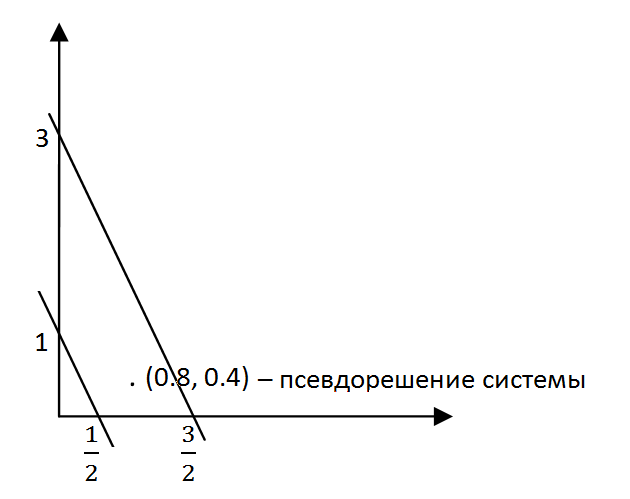
\includegraphics[scale=0.6]{l2_1.png}
\end{center}
\subsection{Сингулярное разложение (SVD)}
\begin{definition}
    $A=Q \Sigma P^*$
    $A: X \to Y$ --- отображение, где $X$ --- размерности $n$, а $Y$ --- размерности $m$.\\
    \[\Sigma = \begin{pmatrix}
    \sigma_1 & 0 & \cdots & \cdots & 0 \\
    0 & \ddots & \cdots & \cdots & 0 \\
    \vdots & \cdots & \sigma_r & \cdots & \vdots \\
    \vdots & \cdots & \cdots & 0 & \vdots \\
    0 & \cdots & \cdots & \cdots & 0 \\
    \end{pmatrix}\]\\
    $Q$ --- ортогональная матрица $m \times m$, 
    $P$ --- ортогональная матрица $n \times n$, 
    $\sigma_1 \geqslant ... \geqslant \sigma_r > 0$.
\end{definition}
Для $A^*A$ существует базис из собственных векторов $e_1,...,e_n$ (где она диагональна).\\
Она неотрицательно определена и существуют собственные векторы $A^*Ae_i=\sigma_i^2e_i$.\\ \\
$
\left\{  
\begin{array}{ccl}  
f_1=\cfrac{Ae_1}{\sigma_1}\\
\cdots\\
f_r=\cfrac{Ae_r}{\sigma_r}\\  
\end{array}   
\right.  
$
\\ \\
$
Ae_i = \left\{\begin{array}{ll}  
\sigma_if_i,& i \leqslant r\\
0,& i > r\\
\end{array}   
\right.  
$
\\ \\
$
A^*f_i=\left\{\begin{array}{ll}  
\sigma_ie_i,& i \leqslant r\\
0,& i > r\\
\end{array}   
\right.  
$
\\ \\
В матрице $Q$ по столбцам стоят векторы $f_1,...,f_r$ (уже получены), $f_{r+1},...,f_m$ (из ортогонализации Грама-Шмидта) в базисе $Y$.\\
$P$ --- столбцы координат $e_1,...,e_n$ в базисе $X$.\\
\\
\textbf{Пример 4.}\\
Найти SVD.\\
\[\tilde{A} = \begin{pmatrix}
1 & 0 & 0 & 1 \\         
0 & 1 & 0 & 1 \\
0 & 0 & 1 & 1 \\
\end{pmatrix}\]
\\
\[\tilde{A}^*\tilde{A} = \begin{pmatrix}
1 & 0 & 0 \\         
0 & 1 & 0 \\
0 & 0 & 1 \\
1 & 1 & 1 \\
\end{pmatrix} \cdot \begin{pmatrix}
1 & 0 & 0 & 1\\         
0 & 1 & 0 & 1\\
0 & 0 & 1 & 1\\
\end{pmatrix} = \begin{pmatrix}
1 & 0 & 0 & 1\\         
0 & 1 & 0 & 1\\
0 & 0 & 1 & 1\\
1 & 1 & 1 & 3\\
\end{pmatrix}\]\\
Найдем собственные значения и векторы $\tilde{A}^*\title{A}$.
\begin{center}
    $\lambda_1=0$\\
    $\lambda_2=1$\\
    $\lambda_3=1$\\
    $\lambda_4=4$\\
\end{center}
Сингулярные числа надо расположить по убыванию.
\begin{center}
    $\sigma_1=\sqrt{4}=2$\\
    $\sigma_2=1$\\
    $\sigma_3=1$\\
    $\sigma>0$\\
\end{center}
\[\Sigma_{3 \times 4} = \begin{pmatrix}
2 & 0 & 0 & 0\\         
0 & 1 & 0 & 0\\
0 & 0 & 1 & 0\\
\end{pmatrix}\]
\\
Найдем собственные векторы.
\begin{enumerate}
    \item $\lambda = 4$\\
    \begin{center}
        $(\tilde{A}^*\tilde{A}-\lambda_iE)x=0$\\
        \[\begin{pmatrix}[r]
        -3 & 0 & 0 & 1\\         
        0 & -3 & 0 & 1\\
        0 & 0 & -3 & 1\\
        1 & 1 & 1 & -1\\
        \end{pmatrix}\cdot x = 0\]
        \\
        $x_1=\cfrac{1}{3}x_4$, 
        $x_2=\cfrac{1}{3}x_4$, 
        $x_3=\cfrac{1}{3}x_4$
    \end{center}
    Получим собственный вектор: \[\begin{pmatrix}
    1\\         
    1\\
    1\\
    3\\
    \end{pmatrix} \cdot c, c\neq 0\]
    \\
    \[e_1 = \frac{1}{2\sqrt{3}} \cdot \begin{pmatrix}
    1\\         
    1\\
    1\\
    3\\
    \end{pmatrix}\]
    \item $\lambda=1$\\
    \[\begin{pmatrix}
    0 & 0 & 0 & 1\\         
    0 & 0 & 0 & 1\\
    0 & 0 & 0 & 1\\
    1 & 1 & 1 & 2\\
    \end{pmatrix} \approx \begin{pmatrix}
    0 & 0 & 0 & 1\\         
    1 & 1 & 1 & 0\\
    \end{pmatrix}\]
    \\
    Получим собственные векторы: \[\begin{pmatrix}[r]
    -1~\\         
    0~\\
    1~\\
    0~\\
    \end{pmatrix} \cdot c_1 + \begin{pmatrix}[r]
    -1~\\         
    1~\\
    0~\\
    0~\\
    \end{pmatrix}\cdot c_2,~ c_1^2+c_2^2>0\]
    \\
    \[e_2 = \begin{pmatrix}[r]
    -\cfrac{1}{\sqrt{2}}~\\         
    \cfrac{1}{\sqrt{2}}~\\
    0~\\
    0~\\
    \end{pmatrix}, e_3 = \cfrac{1}{\sqrt{6}} \cdot \begin{pmatrix}[r]
    1~\\         
    1~\\
    -2~\\
    0~\\
    \end{pmatrix}, e_4 = \cfrac{1}{2} \cdot \begin{pmatrix}[r]
    1~\\         
    1~\\
    1~\\
    -1~\\
    \end{pmatrix}\]
\end{enumerate}
\begin{center} $P=(e_1, e_2, e_3, e_4)$ \end{center}
\[f_1=\frac{\tilde{A}e_1}{\sigma_1}=\frac{1}{2\sqrt{3}} \cdot \begin{pmatrix}
4\\         
4\\
4\\
\end{pmatrix} \cdot \frac{1}{2} = \begin{pmatrix}
\cfrac{1}{\sqrt{3}}\\         
\cfrac{1}{\sqrt{3}}\\
\cfrac{1}{\sqrt{3}}\\
\end{pmatrix} = \frac{1}{\sqrt{3}} \cdot \begin{pmatrix}
1\\         
1\\
1\\
\end{pmatrix}\]
\\
\[f_2=\frac{\tilde{A}e_2}{\sigma_2}=\frac{1}{\sqrt{2}} \cdot \begin{pmatrix}[r]
-1~\\         
1~\\
0~\\
\end{pmatrix}\]
\\
\[f_3=\frac{\tilde{A}e_3}{\sigma_3}=\frac{1}{\sqrt{6}} \cdot \begin{pmatrix}[r]
1~\\         
1~\\
-2~\\
\end{pmatrix}\]
\begin{center} $Q=(f_1, f_2, f_3)$ \end{center}
\[Q = \begin{pmatrix}[r]
\cfrac{1}{\sqrt{3}} & -\cfrac{1}{\sqrt{2}} & \cfrac{1}{\sqrt{6}}\\ \cfrac{1}{\sqrt{3}} & \cfrac{1}{\sqrt{2}} & \cfrac{1}{\sqrt{6}}\\ \cfrac{1}{\sqrt{3}} & 0 & -\cfrac{2}{\sqrt{6}}\\ 
\end{pmatrix}\]
\\
\[\tilde{A} = Q \Sigma P^* = \begin{pmatrix}[r]
\cfrac{1}{\sqrt{3}} & -\cfrac{1}{\sqrt{2}} & \cfrac{1}{\sqrt{6}}\\ \cfrac{1}{\sqrt{3}} & \cfrac{1}{\sqrt{2}} & \cfrac{1}{\sqrt{6}}\\ \cfrac{1}{\sqrt{3}} & 0 & -\cfrac{2}{\sqrt{6}}\\ 
\end{pmatrix} \cdot \begin{pmatrix}
2 & 0 & 0 & 0\\         
0 & 1 & 0 & 0\\
0 & 0 & 1 & 0\\
\end{pmatrix} \cdot \begin{pmatrix}[r]
\cfrac{1}{2\sqrt{3}} & -\cfrac{1}{\sqrt{2}} & \cfrac{1}{\sqrt{6}} & \cfrac{1}{2}\\ 
\cfrac{1}{2\sqrt{3}} & \cfrac{1}{\sqrt{2}} & \cfrac{1}{\sqrt{6}} & \cfrac{1}{2}\\ 
\cfrac{1}{2\sqrt{3}} & 0 & -\cfrac{2}{\sqrt{6}} & \cfrac{1}{2}\\
\cfrac{3}{2\sqrt{3}} & 0 & 0 & -\cfrac{1}{2}\\
\end{pmatrix}^*=\]\\ \[= \begin{pmatrix}[r]
\cfrac{2}{\sqrt{3}} & -\cfrac{1}{\sqrt{2}} & \cfrac{1}{\sqrt{6}} & 0\\ 
\cfrac{2}{\sqrt{3}} & \cfrac{1}{\sqrt{2}} & \cfrac{1}{\sqrt{6}} & 0\\ 
\cfrac{2}{\sqrt{3}} & 0 & -\cfrac{2}{\sqrt{6}} & 0\\
\end{pmatrix} \cdot \begin{pmatrix}[r]
\cfrac{1}{2\sqrt{3}} & \cfrac{1}{2\sqrt{3}} & \cfrac{1}{2\sqrt{3}} & \cfrac{3}{2\sqrt{3}}\\ 
-\cfrac{1}{\sqrt{2}} & \cfrac{1}{\sqrt{2}} & 0 & 0\\ 
\cfrac{1}{\sqrt{6}} & \cfrac{1}{\sqrt{6}} & -\cfrac{2}{\sqrt{6}} & 0\\
\cfrac{1}{2} & \cfrac{1}{2} & \cfrac{1}{2} & -\cfrac{1}{2}\\
\end{pmatrix} = \begin{pmatrix}
1 & 0 & 0 & 1\\         
0 & 1 & 0 & 1\\
0 & 0 & 1 & 1\\
\end{pmatrix}\]
\begin{statement}
        Если $B=AU$, где $U^*=U^{-1}$ унитарная, то $B^+=U^+A^+=U^*A^+$.
\end{statement}
\begin{consequence}
    Если $A=Q\Sigma P^*$, то \[A^+=P\Sigma^+Q^*=P \cdot \begin{pmatrix}
    \sigma_1^{-1} & \cdots & 0 \\         
    \vdots & \sigma_2^{-1} & \vdots \\
    0 & \cdots & \ddots \\
    \end{pmatrix} \cdot Q^*\]
\end{consequence}
\subsection{Линейная регрессия}
\textbf{Модель 1:}\begin{center}
    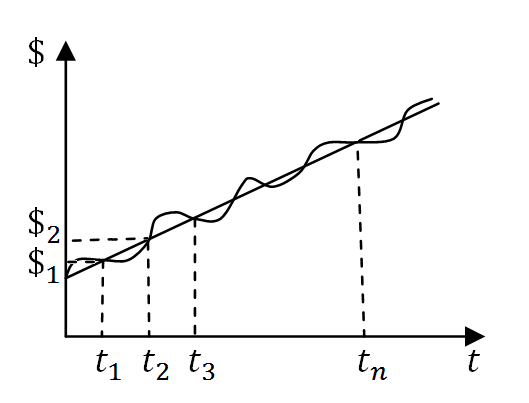
\includegraphics[scale=0.7]{l2_2.png}\end{center}
$\$ = kt+b$\\ \\
$
\left\{  
\begin{array}{ccl}  
\$_1=kt_1+b\\
\$_2=kt_2+b\\
\cdots\\
\end{array}   
\right.  
$\\ \\
Надо найти $k$ и $b$.\\
В матричном виде $A\bar X=\bar S$, где\\
\[X = \begin{bmatrix}
k\\         
b\\
\end{bmatrix}, A = \begin{pmatrix}
t_1 & 1\\         
t_2 & 1\\
\vdots & \vdots\\
t_n & 1\\
\end{pmatrix}, S = \begin{pmatrix}
\$_1\\         
\vdots\\
\$_n\\
\end{pmatrix}\]\\
\[\begin{bmatrix}
k\\         
b\\
\end{bmatrix} = \bar X = A^+\bar S\]\\
\textbf{Модель 2:}\\
Если $x(t)$ --- цена на нефть, то $\$(t)x(t)=k_1t+b_1$.\\
\\
\subsection{Домашнее задание 2}
\begin{enumerate}
    \item
    Доказать утверждение о псевдообратной от произведения матриц.
    Если $B=AU$, где $U^*=U^{-1}$ --- унитарная матрица, а $A$ --- произвольная матрица порядка $n$, то $$B^+=U^+A^+=U^*A^+$$ 
    \item
    С помощью линейной регрессии и псевдообратной матрицы сделать прогноз цены нефти $Br$ в долларах, рублях. Сравнить результаты, полученные с помощью модели 1 и модели 2.
    \item
    Найти SVD для матрицы\\
    \[A=\begin{pmatrix}[r]
    4 & -3i\\
    -3i & 4\\
    \end{pmatrix}\]
    \item
    Найти SVD для матрицы\\
    \[A=\begin{pmatrix}[r]
    6 & 3 & 0\\
    6 & 3 & 0\\
    2 & 5 & 4\\
    -2 & -5 & -4\\
    \end{pmatrix}\]
    \item
    Найти псевдообратную матрицу, используя SVD:\\
    \[A=\begin{pmatrix}[r]
    18 & 18 & 9\\
    4 & -2 & -4\\
    8 & -4 & -8\\
    8 & -4 & -8\\
    \end{pmatrix}\]
\end{enumerate}
~\\